\begin{figure}[H]
\centering
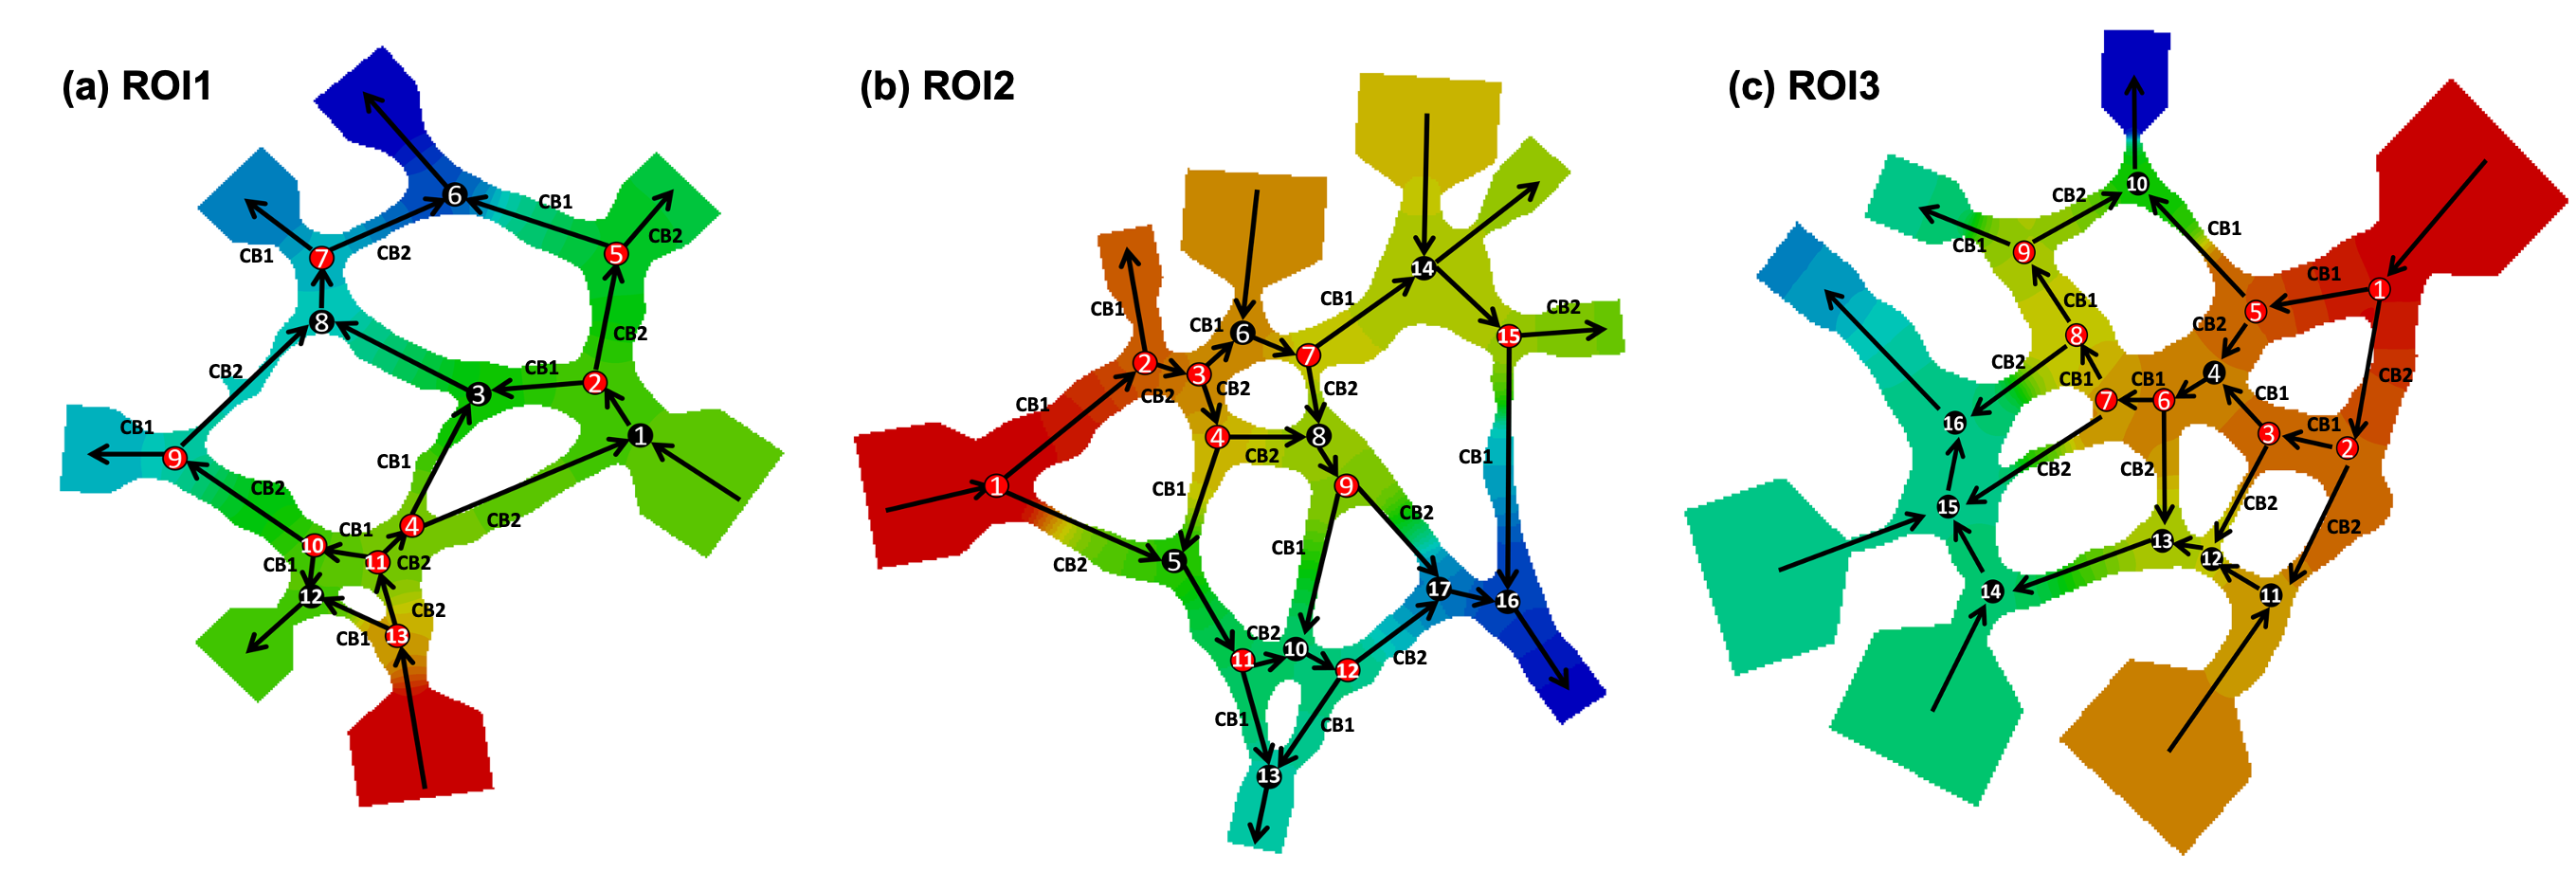
\includegraphics[width=1\textwidth]{images/ROI-Diagrams.png}
\caption{\textit{An illustration of the identified flow patterns and diverging bifurcations within ROI-1, ROI-2 and ROI-3. The diverging and converging bifurcations within each ROI are marked with red and black circles respectively. The arrows represent the direction of blood flow in each individual branch, while the background contour points out the the pressure field where a warmer colour (E.g red) represents higher pressure.} \label{ROIs}}
\end{figure}



% \begin{figure}[H]
% \centering
% \begin{subfigure}{0.33 \textwidth}
%     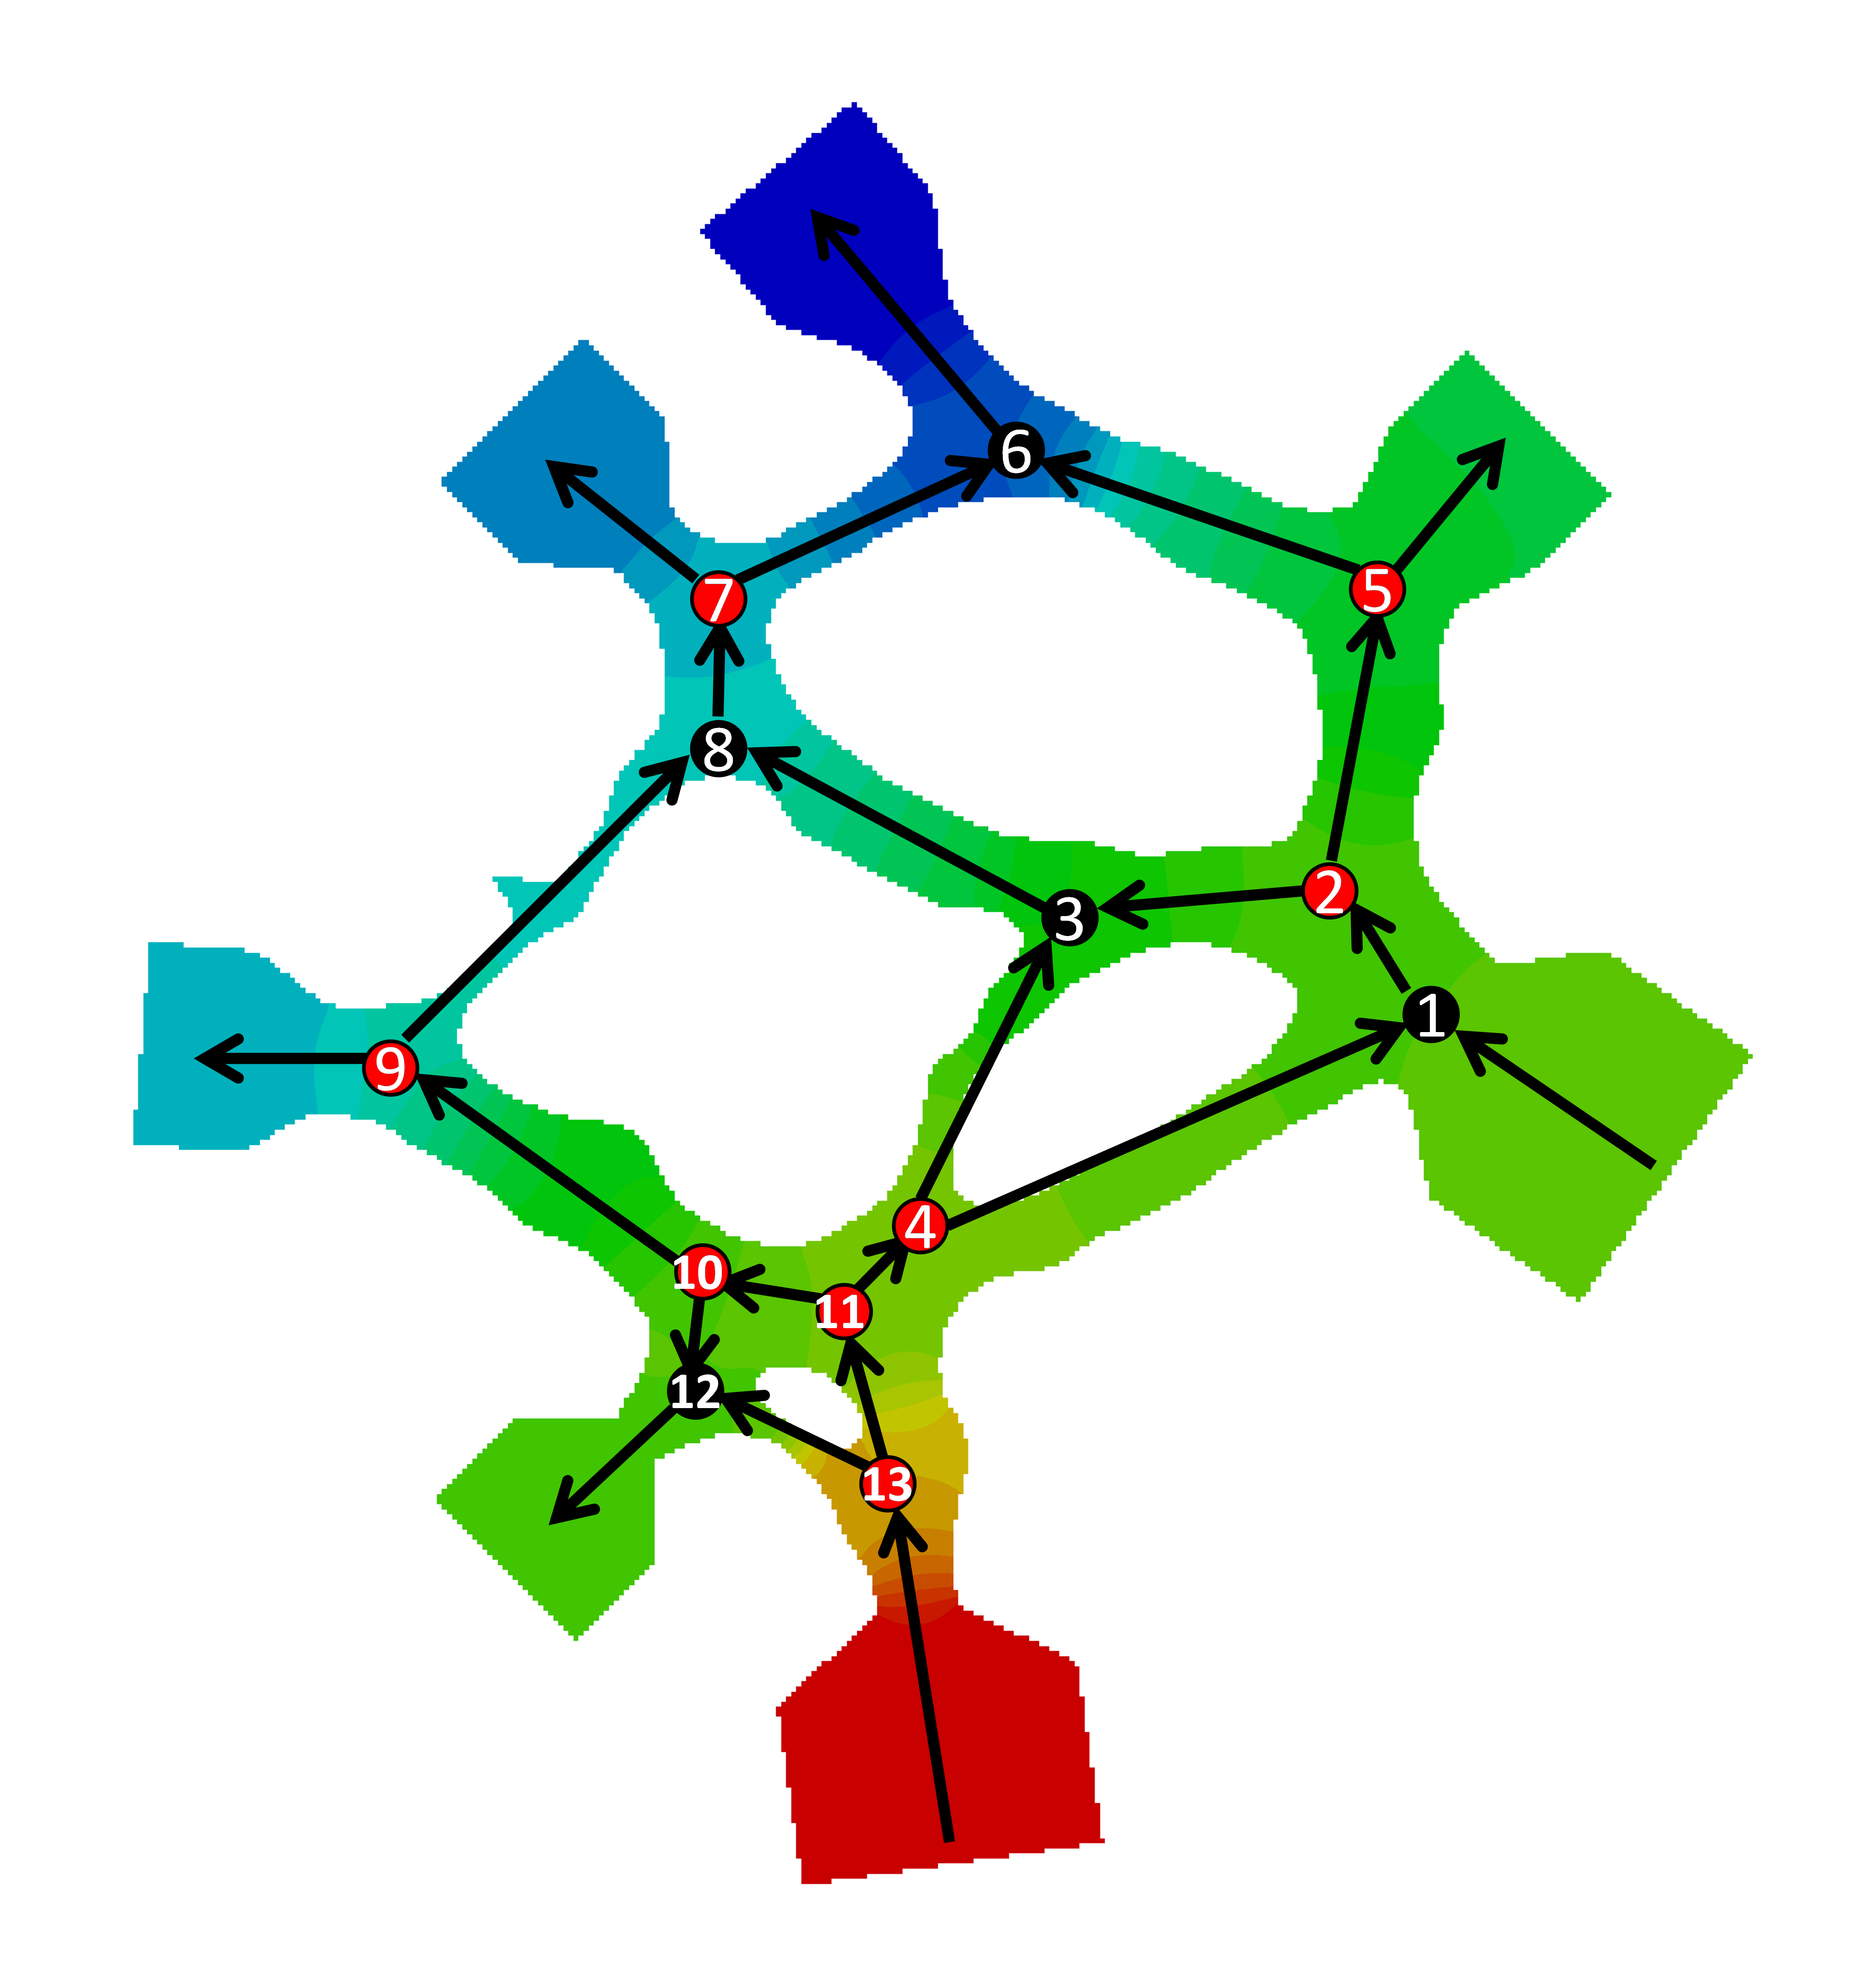
\includegraphics[width=1\textwidth]{images/bifurcations_ROI-1.png}
%     \caption{\textit{Schematic diagram of the ROI1 blood flow network which consists of 8 diverging bifurcations and 19 independent branches.} \label{ROI1}}
% \end{subfigure}
% \hfill
% \begin{subfigure}{0.33 \textwidth}
%     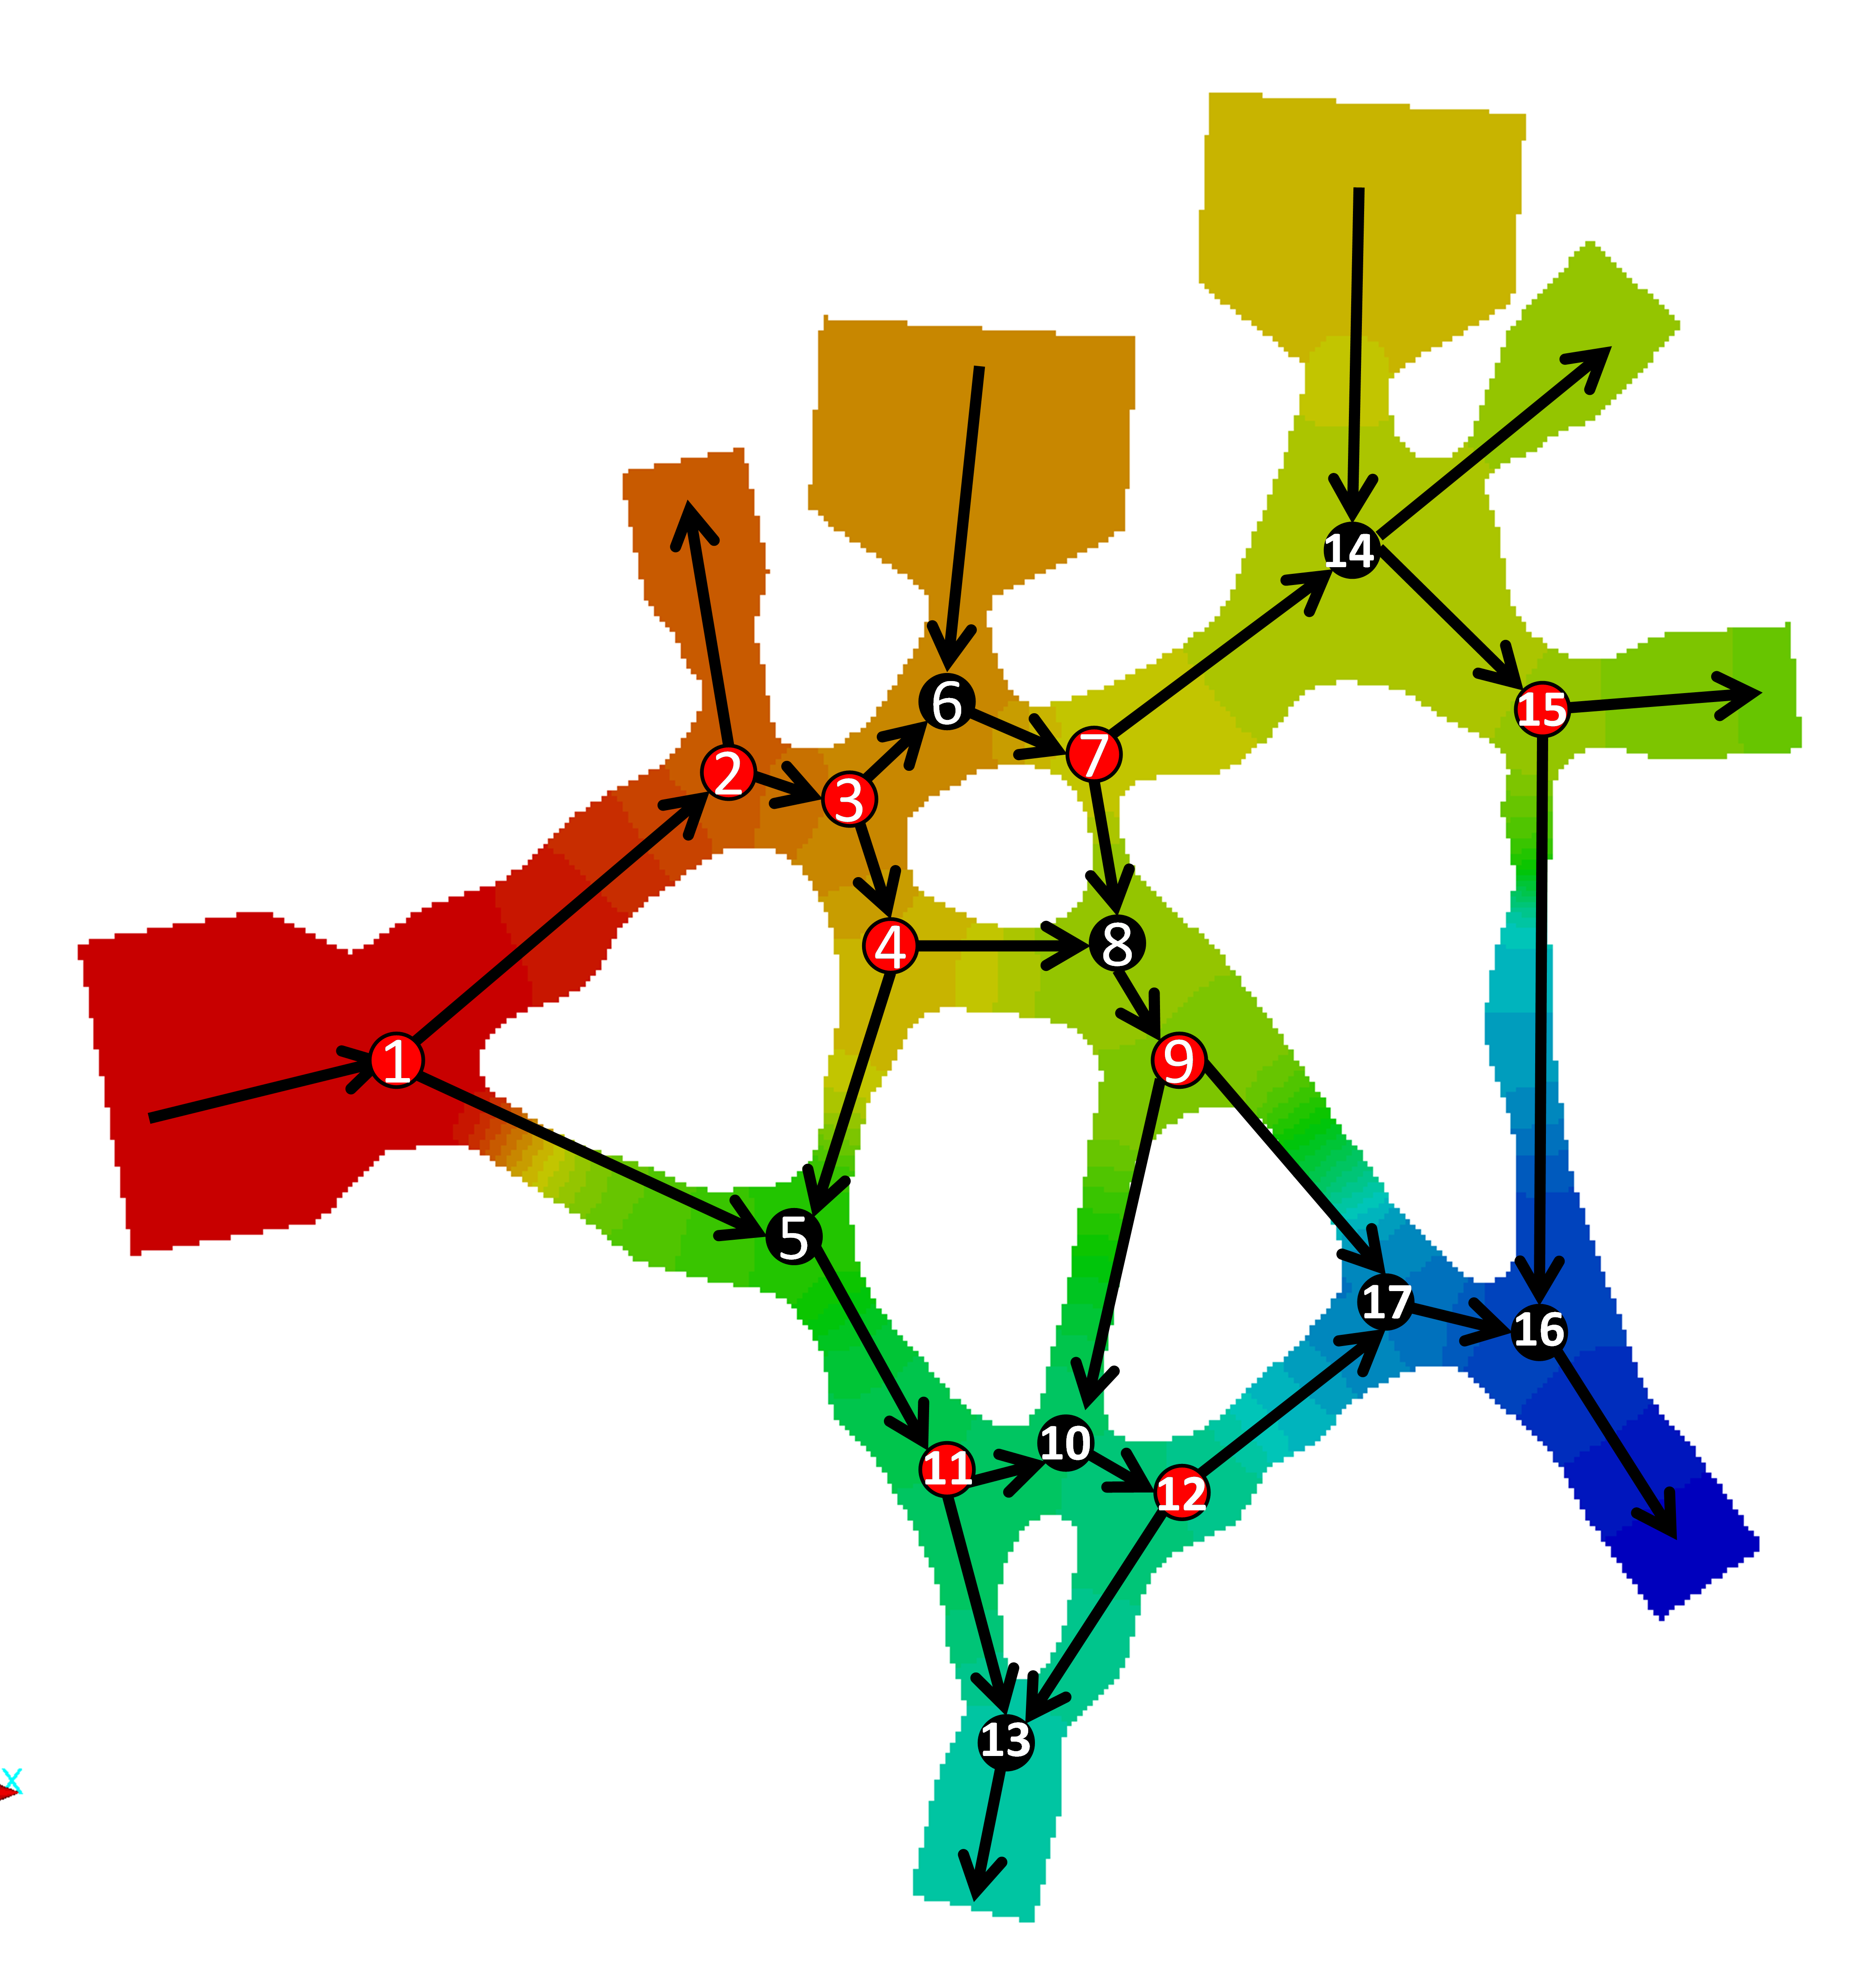
\includegraphics[width=1\textwidth]{images/bifurcations_ROI-2.png}
%     \caption{\textit{Schematic diagram of the ROI2 blood flow network which consists of 9 diverging bifurcations and 24 independent branches.} \label{ROI2}}
% \end{subfigure}
% \begin{subfigure}{0.33 \textwidth}
%     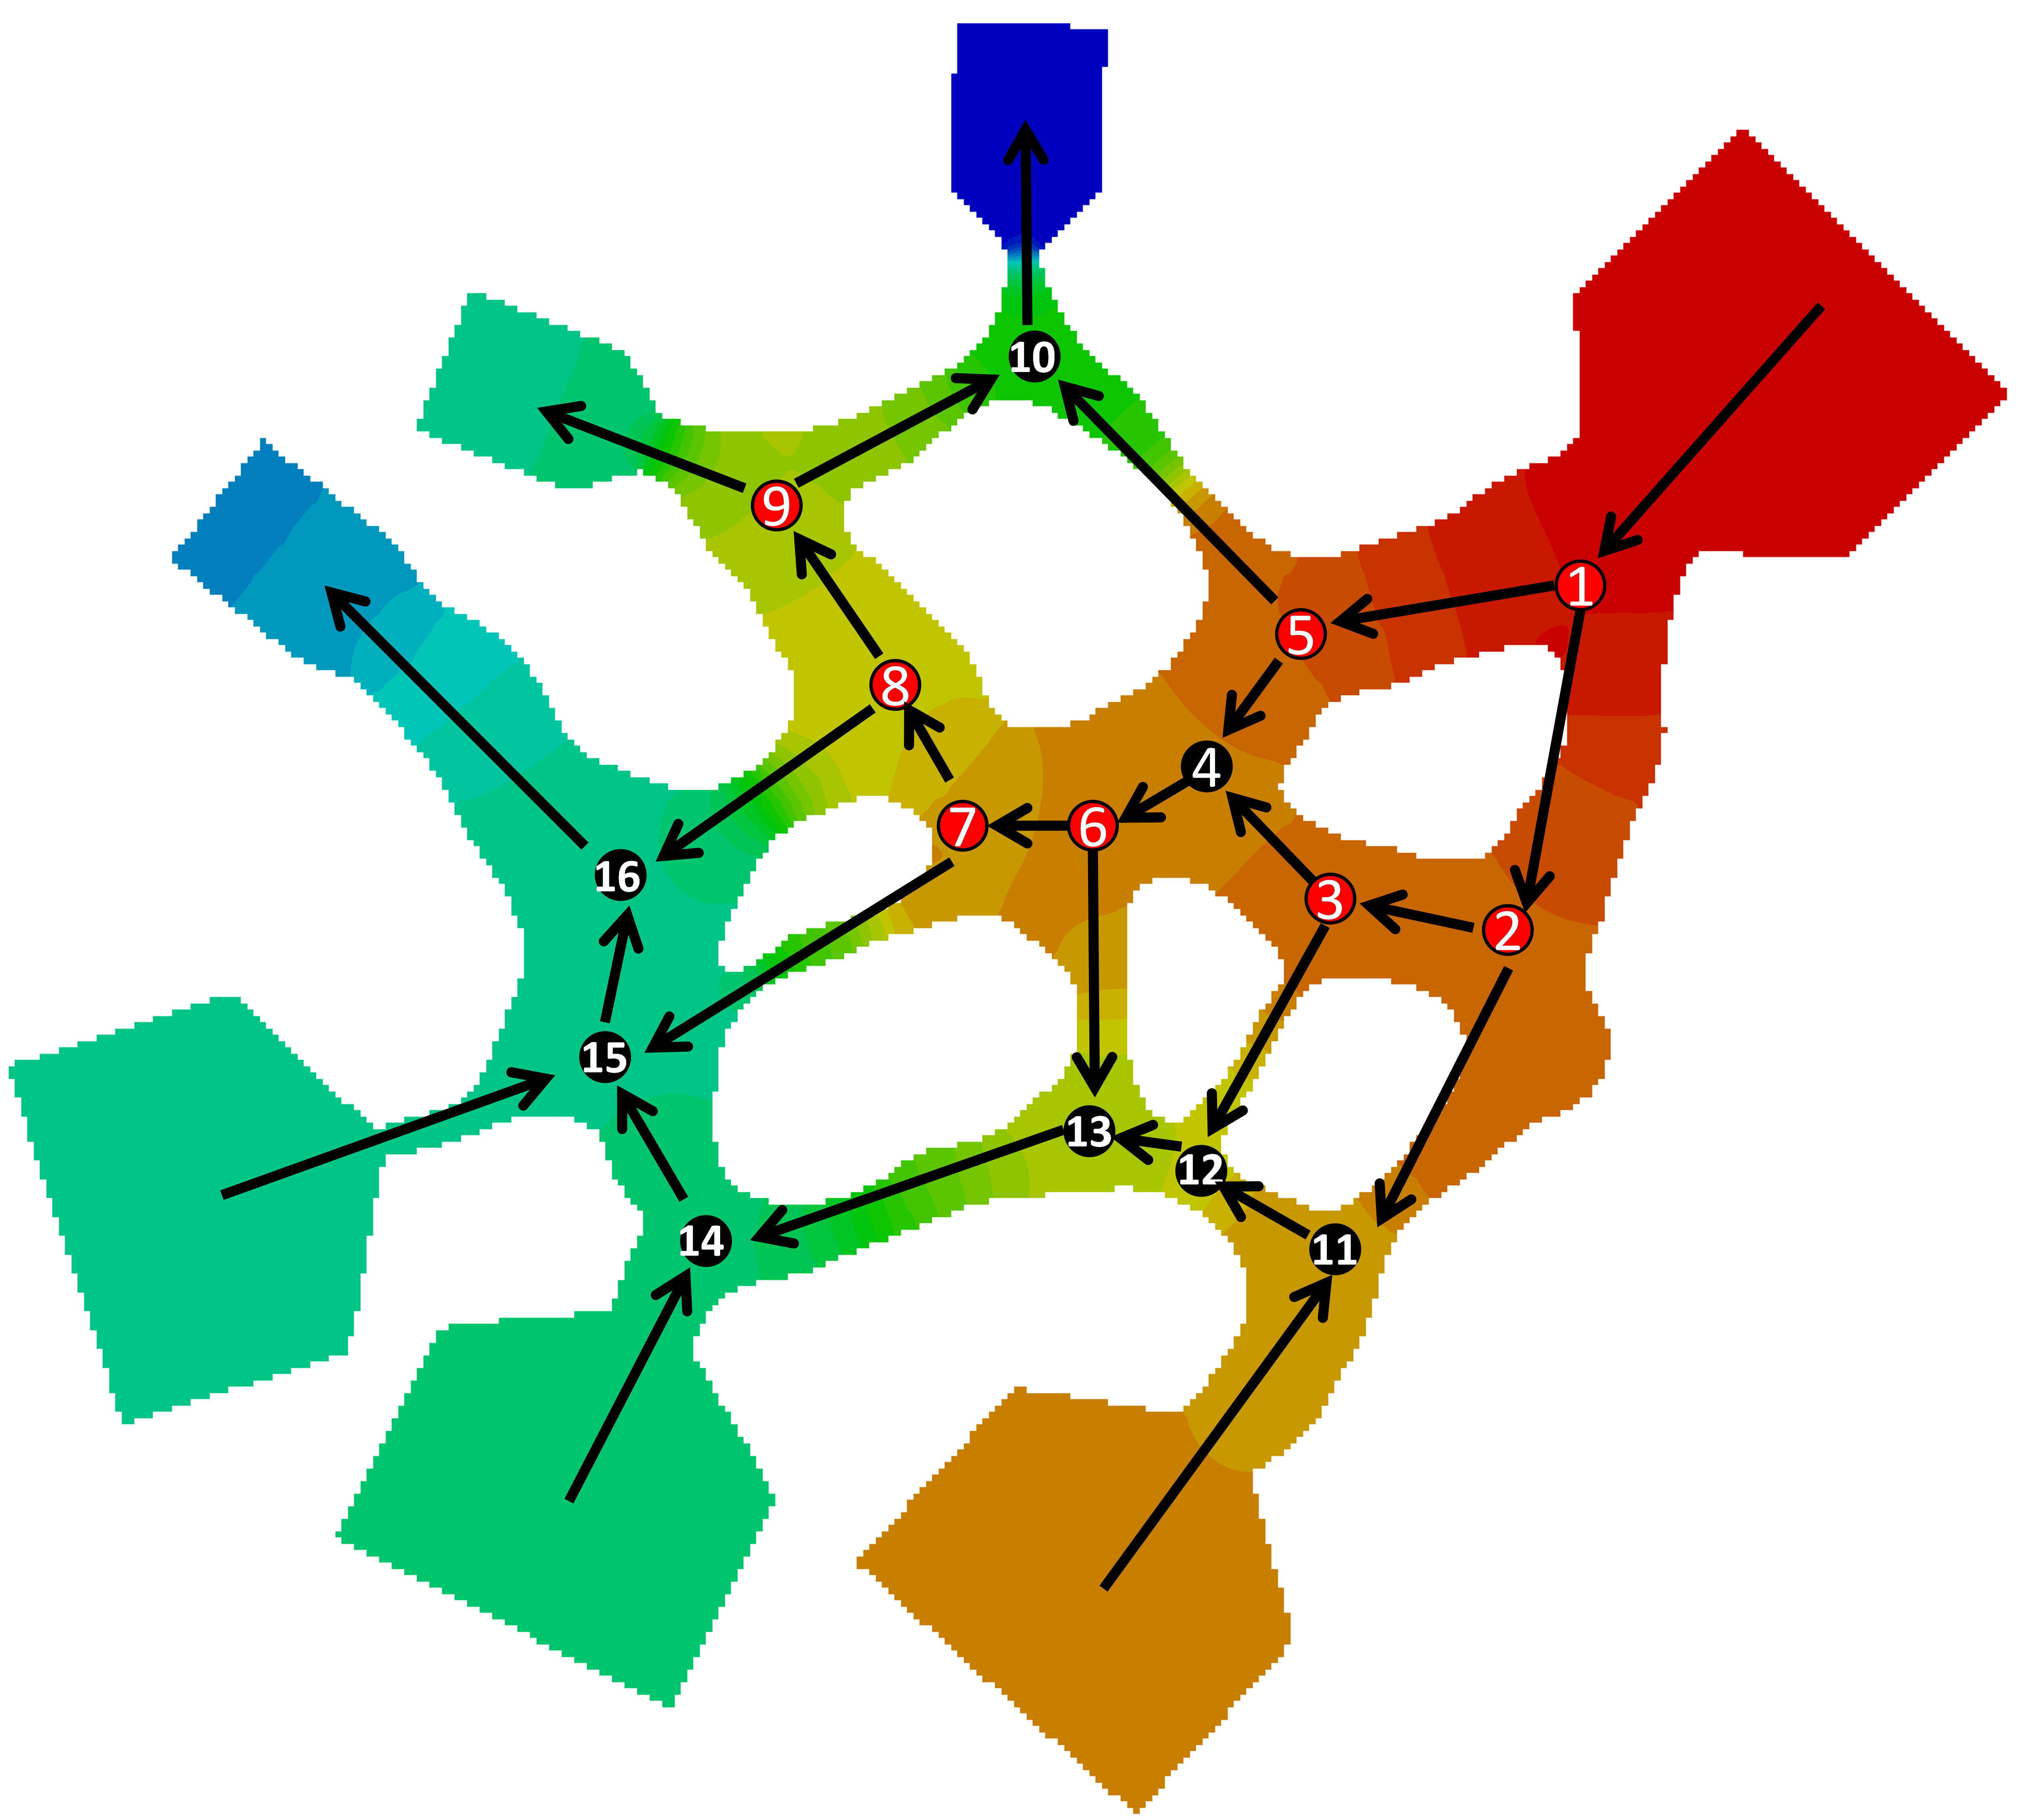
\includegraphics[width=1\textwidth]{images/bifurcations_ROI-3.png}
%     \caption{\textit{Schematic diagram of the ROI3 blood flow network which consists of 8 diverging bifurcations and 18 independent branches.} \label{ROI3}}
% \end{subfigure}
% \caption{\textit{Identification of flow patterns and diverging bifurcations within ROI-1, ROI-2 and ROI-3 respectively. The diverging bifurcations within each ROI are marked with red circles while the converging ones with black. The arrows indicate the direction of the blood flow in each individual branch, while the background contour points out the the pressure field where a warmer colour (E.g red) represents higher pressure.} \label{ROIs}}
% \end{figure}
